\section{Implemented Algorithms}
\subsection{Elimination Tree Data Structure}
\subsection{Heuristics}
\subsubsection{Highest Degree Heuristic}
\subsubsection{Variance Heuristic}
\subsubsection{Bottom-Up Heuristic}
\subsubsection{Formula for lower bound}
We have discovered a function which for given graph $G=(V,E)$ tells us what is a minimum treedepth value for this graph:

\begin{gather*}
f(n,e)=\Bigl\lceil\frac{1}{2}+n-\sqrt{\frac{1}{4}-n+n^2-2e}   \,\Bigr\rceil, \\
\text{where $n = |V|$, $e = |E|$}
\end{gather*}


Here is our thought process.
Let us look at this problem from opposite direction. Given a particular treedepth decomposition, we can create from it all graphs for which this decomposition will be valid. This is pictured on the figure below. As we can see, the treedepth decomposition on the left is a valid decomposition for any graph which has some of the edges shown on the right as a dotted lines. Or in other words: is a valid decomposition for graph on the right and all graphs induced by it.
\begin{center}
	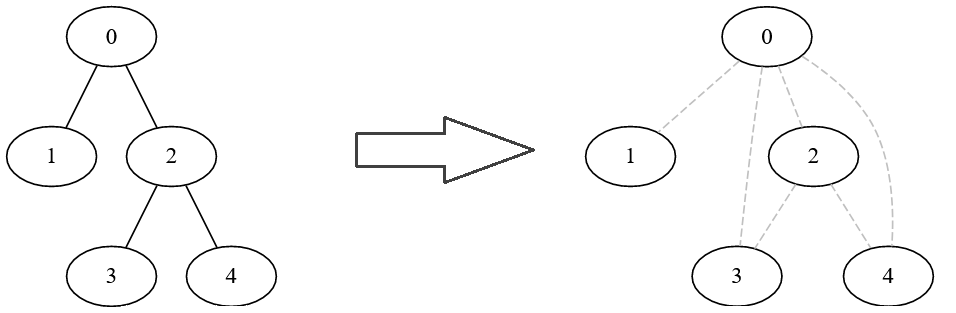
\includegraphics[width=\textwidth]{transform.png}
\end{center}
Here we can notice an important thing: a vertex on level $k$ adds $k-1$ edges that input graph can possibly have. In this example, vertex 3 creates two additional edges that a potential input graph can have: edge 3-0 and 3-2, while vertex 2 - being on level 2 - creates only one additional edge (2-0).\\
Knowing this we can ask ourselves a question: having a fixed treedepth value $td$ and fixed number of vertices $n$, what the structure of treedepth decomposition that maximizes number of possible edges in input graph looks like?\\
Let us carry out the following construction. We start with $n$ vertices and no edges.
At the beggining we do not have any choice as we have to ensure that $td$ equals given value, so we construct $P_{td}$ path. Now we are still left with $n-td$ vertices - where should we attatch them to maximize the number of possible edges in input graph? As we have said earlier: a vertex on level $k$ adds $k-1$ edges that input graph can possibly have. From this we conclude that we have to attatch in such a way that they will be on the lowest possible level which in our case is $k=td$. Below is an example for $td=3$ and $n=5$.
\begin{center}
	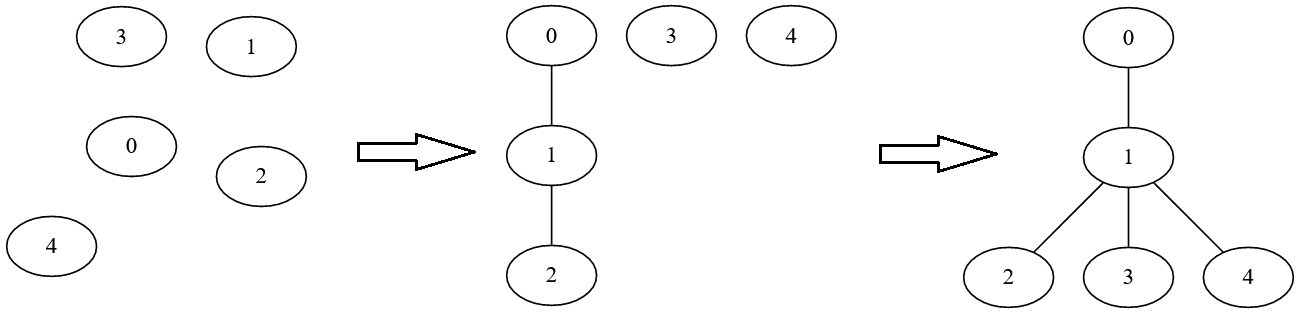
\includegraphics[width=\textwidth]{construction.png}
\end{center}
From all treedepth decompositions with fixed $td$ and $n$, this one supports the highest possible number of edges in input graph. This decomposition supports maximally up to
$$\sum\limits_{i=1}^{td-1} i + (n-td)(td-1)$$edges. The sum part of equation corresponds to the $P_{td}$ path and rest of the equation takes for account the vertices which we attach at the lowest level.\\
Finally, solving this equation for $td$ leaves us with formula presented at the beggining.
\subsection{Exact Algorithms}
\subsubsection{Iterative Dynamic}
\subsubsection{Recursive Dynamic}
\subsubsection{Raw Branch and Bound}
\subsubsection{Branch and Bound with Cache}
